\documentclass[11pt]{article}

\usepackage{fullpage}
\usepackage{graphicx}
\usepackage{url}


\newcommand{\subfigimg}[3][,]{%
  \setbox1=\hbox{\includegraphics[#1]{#3}}% Store image in box
  \leavevmode\rlap{\usebox1}% Print image
  \rlap{\hspace*{0pt}\raisebox{\dimexpr\ht1-0\baselineskip}{\bf
  \normalsize #2}}% Print label
  \phantom{\usebox1}% Insert appropriate spacing
}

\begin{document}

We thank the referees for their assessment of our work.  The following
is our response to each of the specific comments and suggestions.

%%%%%%%%%%%%%%%%%%%%%%%%%%%%%%%%%%%%%%%%%%%%%%%%%%%%%%%%%%%%%%%%%%%%%%%%
\subsection*{Reviewer 1}

The referee wrote: I have reviewed ''Hydrodynamics of Multicomponent
Vesicles Under Strong Confinement'' by Gannon, Quaife, and Young. To my
understanding this work is unique as the dynamics of multicomponent
vesicles under constrictions has not yet been investigated. Before
acceptance there are some questions and issues which should be
addressed:
 
\noindent
{\bf Response:}: We thank the referee for the confirmation that the
topic is unique and has not yet been investigated.

\begin{enumerate}
%%%%%%%%
\item In the phase energy, Eq.~(5), it is stated that the parameter
  $\epsilon$ is much smaller than 1 but then it is stated that this
    parameter is equal to 100. Please address this inconsistency.

\noindent
{\bf Response:} This was a typo. We checked our code, and now we
report the correct value in the revision which is $\epsilon = 0.04$.

%%%%%%%%
\item What motivated the choice of a sigmoid function, Eq.~(9), rather
  than a simple min/max operation so that the bending rigidity does not
    extend past the $[0.1, 1]$ range? Would the use of a regular-mixture
    model, which might be more physically realistic, remove the need for
    such a mathematical approximation as the equilibrium concentrations
    will no longer be $0$ and $1$?

\noindent
{\bf Response:} Because we are using an integral equation formulation,
    we are able to achieve high-order accuracy as long as everything is
    smooth, including the vesicle shape, tension, and the bending
    stiffness. If we used any kind of $\max$ or $\min$ function, the
    bending modulus would lose differentiability and this would result
    in a loss of accuracy. We have expanded the text to explain this
    point.

    We are unsure what the reviewer means by a ``regular-mixture model".
    If they mean a linear parameterization between the stiff and floppy
    phases, this is exactly equation (8).  We originally used this
    choice, but as argued in the manuscript, because of the strong
    confinement, the lipid concentration could easily exceed a value of
    $1$, and this resulted in a unphysical negative bending modulus
    which ultimately leads to an instability.  Figure 2 demonstrates
    this effect. Furthermore, Figure 3 validates the choice of the
    sigmoid parameterization by comparing the results with a result from
    the literature that used the linear parameterization in an unbounded
    linear shear flow.

%%%%%%%%
\item Please define $\eta$ in Eq.~(10). 

\noindent
{\bf Response:} $\eta$ is the stress density that is used to satisfy the
    Dirichlet boundary condition on the solid walls. The text has been
    adjusted.

%%%%%%%%
\item Please define whether $\mathbf{n}$ in Eq.~(12) is the inward or outward pointing unit normal.

\noindent
{\bf Response:} It is the outward pointing unit normal.  We have adjusted the text to clarify this.

%%%%%%%%
\item How is surface incompressibility enforced?

\noindent
{\bf Response:} The surface incompressibility is enforced via the tension $\sigma$ (Eq.~(6)) in the original manuscript), 
which is a Lagrange multiplier so that the inextensibility condition can be satisfied. We adjusted the text in the revision to make this clearer.

%%%%%%%%
\item Please define $\mathbf{U}$ in Eq.~(15). Is this the velocity of
  the interface?

{\bf Response:} This is the prescribed velocity along the solid wall
    which is a combination of no-slip along the top and bottom of the
    channel, and a Poiseuille flow at the inlet and outlet. We now
    reference equation (3), which defines $\mathbf{U}$, immediately
    after equation (15). 

%%%%%%%%
\item What value of $\delta$ is used to determine the lubrication layer
  thickness?

{\bf Response:} We used the dimensionless value $\delta = 0.3$. For the
stenosis geometry, this corresponds to a lubrication layer thickness of
a little more than one micron. This value is now mentioned in Section
2.4.

%%%%%%%%
\item The simulation parameters must be provided. In the stenosis case
  what is the (dimensionless) width of the constricted region? For the
    contracting geometry case what does a $2~\mu$m wide neck correspond
    to?

{\bf Response:} We now report the dimensionless width of both
geometries.

\end{enumerate}

\newpage 
%%%%%%%%%%%%%%%%%%%%%%%%%%%%%%%%%%%%%%%%%%%%%%%%%%%%%%%%%%%%%%%%%%%%%%%%
\subsection*{Reviewer 2}

The referee wrote: The authors of the paper, explored the effect of
hydrodynamics on the behavior of multicomponent vesicles under strong
confinement using numerical simulations. They have elucidated the
effects of the lubrication layer that exists between the vesicle, and
explored how confinement affects the excess pressure needed to push the
vesicle through the conduit. This study is useful to the community and
contains some sound insights regarding multicomponent vesicles. It,
however, is important that the authors make the following changes to be
considered for publication.

\noindent
{\bf Response:}: We thank the referee for their assessment and suggested
changes.

\begin{enumerate}
%%%%%%%%
\item The authors specify a line energy parameter $\epsilon = 100$. It
  is important that the authors justify this choice along with an
    experimental study which uses similar parameter ranges. This is
    important so that a future experimental study could be performed
    using these parameters as a guide.

\noindent
{\bf Response:} This was a typo. We checked our code, and now we
report the correct value in the revision which is $\epsilon = 0.04$.
This value corresponds to a transition region of size $10^{-1}$ microns
between stiff and floppy regions. Comparable values are used in the
literature, and we cite three of these papers.

%%%%%%%%
\item Minor comment: In Figure 4 and 5, the authors should add the $x$
  coordinate under the figure so that the readers are able to understand
    the results better.

\noindent
{\bf Response:} Thank you for the suggestion. The $x$ coordinate is
added to these figures in the revised manuscript.

%%%%%%%%
\item The authors mention the phrase `size of lubrication layer' in the
  paper. They need to explicitly define this parameter. It could be
    confusing to a reader whether they talk about
    $|\gamma_{\mathrm{layer}}|$ or $w_{\mathrm{top}}$ and
    $w_{\mathrm{bottom}}$.

\noindent
{\bf Response:} We have labelled $w_{\mathrm{top}}$ and
$w_{\mathrm{bot}}$ in Figure 1. We have adjusted the text in Section
2.4.

%%%%%%%%
\item The authors measure the tangential velocity at 4 points. They
  should provide some justification for this number. Also, it is
    advisable that in Figure 7, the authors use a different color for
    each velocity plot. The plot looks highly convoluted and does not
    convey the message clearly. Also, what are the bounds within which
    the authors call the tangential velocity to be constant in Figure 7?
    They should define a bound for the variation that could be
    considered constant. Moreover, in Figure 7, for the floppy vesicle,
    the authors see a large deviation for the tangential velocity. It
    doesn't seem like the velocity could be called `constant'. The
    authors should provide a more detailed explanation for this.

\noindent
    {\bf Response:} We calculated the tangential velocity of all $N =
    1024$ Lagrangian points for each of the three cases. Plotting all
    1024 lines in the manuscript would be uninformative. To prove this is
    the case, a plot of 32 of the tangential velocities is in Figure~\ref{fig:tangVel} of this document. 
%    
Instead we track the tangential velocity of each Lagrangian marker on
the vesicle membrane, measuring the spread in this tangential velocity
over the part of the period when the vesicle is inside the stenosis.
This spread, scaled by the velocity magnitude, is color-coded along the
membrane and is now part of Figure 7. The original plots showing the
tangential velocity of the four points are removed. For a tank-treading
vesicle, this scheme would give a membrane of a uniform color. On the
other hand, a non-uniformly colored membrane implicates the lack of
tank-treading in the vesicle membrane, which may also correspond to
significant deformations in the membrane.
%   
% Instead, in the document,
%  we report the average tangential velocity in the region $x \in
% [4,10]$, and report the spread of all tangential velocities from
%this mean value. 
More quantitatively, if this spread is less than 15\%, we would
characterize this as a tank-treading vesicle. Their spread is 1.2\% for
the stiff single-component vesicle, 12\% for the multicomponent case,
and 313\% for the floppy single-component case. Therefore, the floppy
single-component vesicle is not tank-treading, while the other two cases
are tank-treading. We have made this clear in the text.

\begin{figure}[ht]
  \centering
  \subfigimg[width=0.3\textwidth]{(a)}{figures/SC_treading_velocity_review.pdf}
  \subfigimg[width=0.3\textwidth]{(b)}{figures/SCp55_treading_velocity_review.pdf}
  \subfigimg[width=0.3\textwidth]{(c)}{figures/MCp5_treading_velocity_review.pdf}
  \caption{\label{fig:tangVel} The tangential velocity of 32 points of
  the (a) stiff single-component vesicle, (b) floppy single-component
  vesicle, (c) multicomponent vesicle. Note that these figures, and the
  version with four marker points, are excluded from the revised
  manuscript.}
\end{figure}

%%%%%%%%
\item In some simulations, the authors choose a `random' initial
  condition. It would be helpful if they could mathematically define the
    function for this initial condition.

\noindent {\bf Response:} The examples with a random initial condition
use the uniform distribution with the range $[0,1]$ to define the lipid
concentration $u$ at each spatial point. Given the choices of
$b_{\min}=0.1$ and $b_{\max}=1$, the resulting mean bending stiffness is
$\overline{b(u)} \approx 0.55$. The text has been adjusted at the start
of Section 3.1 and Section 3.2.

%%%%%%%%
\item In Figure 6, the author should comment on the energy behavior of
  the floppy vesicle in the stenosis region.

\noindent
{\bf Response:} We have included a discussion of the energy behavior of
the floppy vesicle and compared it with the stiff case.

%%%%%%%%
\item In Figure 7, when the authors look at the excess pressure plots,
  they should describe the behavior of the floppy vesicle due to the
  difference in lubrication thickness and, in turn, excess pressure. It
  seems like the excess pressure shows a similar trend as the stiff
  vesicle.

\noindent
{\bf Response:} In the original submission, we attempted to relate the
excess pressure to the lubrication layer thickness. However, as pointed
out by the reviewer, we did not make any reference to the floppy case.
As a general trend, we find that the sum of the top and bottom
lubrication layer thicknesses is correlated with the magnitude of the
excess pressure---larger lubrication layers correspond to smaller (less
negative) excess pressures. This is because smaller excess pressure is
required to push the same amount of fluid around the vesicle when the
lubrication layer thickness is larger. The text has been adjusted.


%%%%%%%%
\item Not really a comment, but the author's analysis of the velocity
  profiles in Figure 8 is fantastic. It captures the stress and pressure
  gradient behavior aptly and provides a theoretical basis as well.

\noindent
{\bf Response:} We thank the reviewer for this compliment. We are also
very happy with this result. 


%%%%%%%%
\end{enumerate}

\newpage

%%%%%%%%%%%%%%%%%%%%%%%%%%%%%%%%%%%%%%%%%%%%%%%%%%%%%%%%%%%%%%%%%%%%%%%%
\subsection*{Reviewer 3}

The referee wrote: The authors study the passage of a vesicle through a
constriction. A vesicle’s membrane has some mechanical properties analog
to red blood cells motivating many theoretical and numerical studies.
Indeed, this issue has known many progress during the last decade. A
vesicle is also a fascinating physical soft particle as its membrane
area is constant as well as its volume leading to an essential role of
deflation. But contrary to capsules, as the membrane is fluid, there is
no buckling. Finally, the study is inspired by modeling RBC. 

\noindent
{\bf Response:} We thank the referee for their assessment and suggested
changes.

\begin{enumerate}
%%%%%%%%
\item This study is limited to the two-dimensional case, which is not
  reality. It is a strong approximation and full 3D studies are still a
    challenge in constrictions. But, in the axisymmetrical case, there
    are several results in literature which could be more or less,
    considered as benchmark:
    \url{http://dx.doi.org/10.1103/PhysRevFluids.5.043602}, \\
    \url{https://doi.org/10.1017/jfm.2017.743}

\noindent
{\bf Response:} Thank you for the comment. It is addressed in detail in
our response to the reviewer's second comment.

%%%%%%%%
\item The authors should justify why they limit their investigations to
  the 2D case if 3D is possible. I note that the authors also cite
    relevant literature as 10, 11 $\ldots$ References to 2D are
    excellent. A typical argument is the high time of 3D simulations.
    Can the authors provide an order of magnitude?

\noindent
{\bf Response:} There is published work that has investigated elements
of our work in  3D. This includes the papers from the reviewers first
comment that consider vesicles in strong confinement, but these works
assume axisymmetry and neither consider multicomponent vesicles. Two 3D
works that relax the axisymmetric assumption and simulate vesicles in
strong confinement are also cited in the original submission
(https://doi.org/10.1063/1.5081057 and
https://doi.org/10.1103/PhysRevFluids.5.013603). Red blood cells
undergoing strong confinement has also been considered using other
numerical methods including a spring model coupled to smoothed particle
hydrodynamics (http://dx.doi.org/10.1016/j.taml.2015.11.006 and
http://dx.doi.org/10.1063/1.4817959). These papers are cited in the
revised manuscript.

There is much less work on 3D multicomponent vesicles. Phase field
models are used by Wang and Du
(https://doi.org/10.1007/s00285-007-0118-2) and a level set method is
used by Gera and Salac
(https://doi.org/10.1016/j.compfluid.2018.04.003). The challenge with
both these approaches is that they have to discretize the fluid volume,
and this limits how small $\epsilon$ can be, and therefore restricts
the sharpness of the transition between the floppy and stiff
regions. In both these works, a value of $\epsilon$ that is at least
ten-times larger than the more realistic value used in our work. To use
a comparable value to ours, they would have to increase the overall
spatial resolution by $10^3$. These codes are parallelized and highly
optimized, but they still take on the order of a day to complete one
unconfined simulation at the coarser resolution. Therefore, with
confinement, and the additional resolution to resolve the more physical
value of $\epsilon$, a single simulation would require much more
computational resources for generating an appropriately large dataset to
analyze. For example, if a simulation for an unconfined case requires
one day of CPU time on 12 cores, then, even without confinement, the
additional resolution required to resolve the smaller value of
$\epsilon$ would require 12,000 cores to complete the simulation in the
same wall clock time, and this is assuming the code scales perfectly.
This increase in resources would be compounded further once strong
confinement is introduced.

Extending our 2D spectral code to 3D is challenging because resolving
the sharp interface between lipid domains requires special treatment
such as adaptive methods. Recently, finite element methods with adaptive
mesh generation have been used to solve surface PDEs, but to our
knowledge, it has not been extended to fourth-order PDEs or evolving
surfaces (as in our case). For example, see the following thesis that
considers reaction-diffusion systems on surfaces
(https://nrs.harvard.edu/URN-3:HUL.INSTREPOS:37368862), and the preprint
written by the same author (https://arxiv.org/pdf/2210.00022.pdf).
Extending this work to incorporate a high-order phase field model and
deformable interface is currently unavailable, to the best of our
knowledge.


%%%%%%%%
\item The authors present the essential steps of the numerical model. It
  is well done and the references well chosen. I have appreciated the
    introduction of equation (9) an figure 2. However, there are two
    points to clarify :
    \begin{itemize}
      \item page 2: there is a difference in literature of the
        capillary number. Some authors use the flow curvature, others
        the mean velocity as the authors. Please explain your choice.
      \item page 2, right column ``The parameter $\epsilon \ll 1$ sets
        the size of the transition region of u, and the parameter a is
        line tension scaled by the characteristic bending stiffness. All
        simulations use the parameter values $\epsilon = 100$ and $a =
        0.04.$" $\epsilon = 100$ is contradictory to $\epsilon \ll 1$.
        Please explain or correct
    \end{itemize}

\noindent
{\bf Response:} We use the maximum imposed velocity to define the
capillary number so that we can compare our results with work that we
cite including [10,11,18] (as numbered in our original submission). We
have also added a note that the capillary number is larger for a vesicle
inside the stenosis.

For the comment regarding the value of $\epsilon$, we had a
typo. The parameter value for $\epsilon$ is actually 0.04, and this has
been fixed.

%%%%%%%%
\item Why do authors never observe the blocking of vesicles contrary to
  experiments? It would the opportunity to perform a phase diagram and
    to show the effect of multicomponent.

\noindent
{\bf Response:} We initially explored cases where the single-component
vesicle became stuck, expecting that the multicomponent vesicle may pass
through the same geometry. We did not find any such cases.
However, we did observe other behaviors that differ between the two
cases, including the vesicle shape, tank treading velocity, lubrication
layer, and these comparisons are the focus of our manuscript. We defer
our response to the phase diagram point until comment number 6.

%

%%%%%%%%
\item In experiments, the channel is a slit. What do the authors expect
  from such a difference?

\noindent
{\bf Response:} We are interpreting this question as the reviewer asking
about 3D effects. In the literature, the 3D simulations of a red blood
cell through a 3D slit (see Lu and Peng,
https://doi.org/10.1063/1.5081057) has a 2D projection that looks
similar to our 2D simulations. In particular their right-most panel in
Figure 5(b) resembles Figures 10(d) and 10(e) in columns V and VI from
our paper. Other than the shape similarity of the 2D projection, we also
find that our excess pressure is of the same order for a similar flow
rate in a 3D case (http://dx.doi.org/10.1063/1.4817959).

%%%%%%%%
\item Finally, this study is interesting and provides new insights.
  However, I advise authors to improve the quantitative part of their
  results (variation with Ca or confinement or something else, phase
  diagram...) to be more relevant for a journal such as Soft Matter. I
  am waiting the new manuscript.

\noindent
{\bf Response:} As shown recently by Agarwal and Biros
(http://www.doi.org/10.1103/PhysRevFluids.5.013603) (see Figure 18a),
when a vesicle is in a channel with strong confinement, there are at
most two different shapes a vesicle can take on for different capillary
numbers. They observe this for confinement ratios as large as 0.7, and
our examples have a confinement ratio closer to 2 (stronger
confinement). To verify this claim, we constructed a phase diagram for a
multicomponent vesicle in a unconfined non-linear shear flow by varying
the reduced area and the capillary number. We observe that the
multicomponent vesicle is more symmetric in shape than the
single-component vesicle for a wide range of capillary numbers and
reduced areas (Figure~\ref{fig:Phase}). Based on this, we speculate that
a phase diagram with strong confinement would be less interesting than
the single-component case, so we exclude a phase diagram in confinement.
%
%A phase diagram is included in Figure~\ref{fig:Phase}.
%We do not observe any dependence on the capillary number. 

We have also discussed this topic with a colleague who works on
experiments with a red blood cell passing through stenosis, where RBCs
form a single line in the mid-plane of the channel. His experiments have
shown that the shape of the RBC inside this confined stenosis is
independent over a range of capillary numbers. For this reason, we focus
on the relationships between between the vesicle shape, lubrication
layer, excess pressure, and asymmetry relative to the midline.

We have started examining the dependence of the vesicle symmetry on
other dimensionless parameters such as the confinement ratio and the
floppy-to-stiff ratio. This will likely give rise to different phenomena
and analyses that would distract from the focus of this work.
\begin{figure}
\centering
  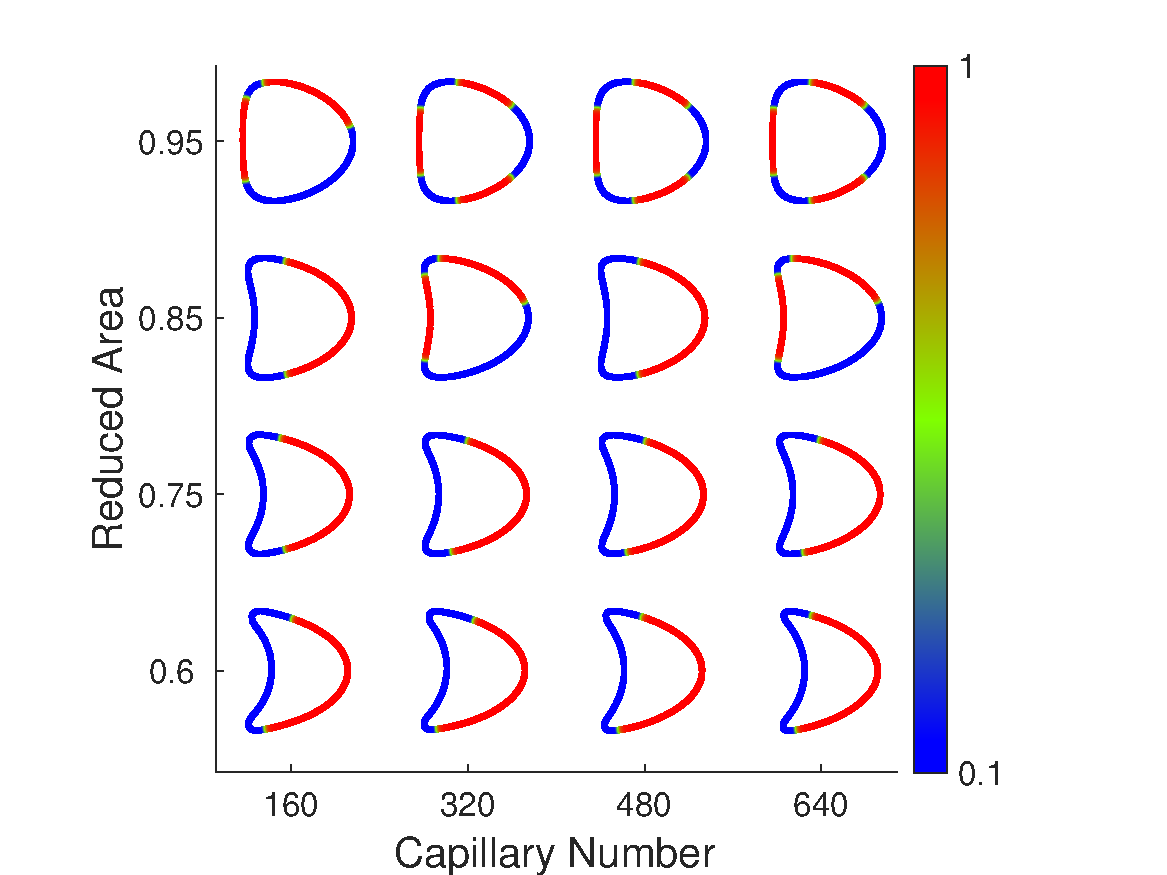
\includegraphics[width=0.5\textwidth]{phaseDiagram.pdf}
  \caption{\label{fig:Phase} A phase diagram of a single multicomponent
  vesicle in an unconfined nonlinear shear flow. The capillary number
  has no effect on the steady state shape of the vesicle.}
\end{figure}

%%%%%%%%
\item Page 2, left column : the flow is assumed to be in the limit of
  zero Reynolds number : not the fluid

\noindent
{\bf Response:} Thank you for correcting this error. We have added the
word `flow' to the manuscript.

%%%%%%%%
\item The title is a bit misleading as the authors only consider the
  deflation equal to the one of RBC. However, as there is some conflict
  between capsules and vesicles as models of RBC, the title can be
  tolerated.

\noindent
{\bf Response:} We thank the referee for this comment. We did not change the title as the referee found it tolerable.
\end{enumerate}


\end{document}
